\documentclass[12pt, letterpaper]{article}
\usepackage[utf8]{inputenc}
\usepackage[margin=1in]{geometry}
\usepackage{graphicx}
\usepackage{xurl}
\usepackage{courier} %% Sets font for listing as Courier.
\usepackage{listings, xcolor}
\lstset{
basicstyle=\tiny ,
tabsize = 4, %% set tab space width
showstringspaces = false,
numbers = left,
commentstyle = \color{gray},
keywordstyle = \color{blue},
stringstyle = \color{red},
rulecolor = \color{black},
basicstyle = \small \ttfamily ,
breaklines = true,
numberstyle = \tiny ,
xleftmargin=0.55cm
}

\title{COMP3340: Final Project Submission \\{New City Better Life | Project Team 9}}
\author{Pao Yu | Chen Qiao | Weichong Wu | Yijiu Xu}
\date{University of Windsor | 13/08/2021}
\begin{document}
\maketitle

\begin{abstract}

    \textbf{Summary}
    \textit{New City Better Life.} Almost one quarter of Canadians moved or plan to move since April 2020. These survey participants cited COVID-19 as a reason for relocating. We started \textit{New City Better Life} as a way to help this market do their research on possible dream cities so that they can relocate to any city in Canada. On our website, you may get information on 166 of the most livable cities/towns in Canada.
    
    \textbf{Purpose}
    The purpose of our website is to help people who have a plan to move in the future. We provide key livability statistics and information on almost all cities and towns in Canada that can be saved by users and help them make decisions regarding their relocation in the future.
   
    \textbf{Methodology}
    This website was created using the standard LAMP-stack (Linux, Apache, MySQL, and PHP). The front-end is built with HTML, CSS and JavaScript. The project was initially created by carefully planning a sitemap using the project's purpose and background. From this sitemap, we implemented the most important pages by the predicted frequency of use by our potential users, with the index page being the highest priority page to have been implemented. After the most important pages were created (and connected through a working navigation system), we then turned our efforts to the heart of the website's functionality, which was to be able to display database records on dynamic PHP pages and a working login system for admins and clients.

    \textbf{End Result}
    At the end of the semester, we completed an MVP website with the core functionalities and requirements that was needed to make the site operational. It is currently live and running, with users able to register, login and use the site to search for information related to their dream city, while being able to maintain a data-persistent, account-based list of their favorite cities through a logged-in account. The website is also highly-maintainable on the admin side, with high quality documentation for both end-users and admins. Finally, our website and code is open-source on GitHub and is ready to be cloned, deployed and installed by third-party developers who would like to implement our codebase to build similar projects in the future.

\paragraph*{Contribution: } All team members contributed equally for this project.

\end{abstract}

\newpage

\tableofcontents

\newpage

\section*{Client Interface Checklist}

% =====================================================================
%   1. LANGUAGES USED
% =====================================================================
\section{Languages Used}
e.g. HTML5, CSS3, JavaScript, PHP, etc..

In your report, for each item using the corresponding section number from the table above to present/expand on the work you have done. You can include code segments, screenshots and charts as needed for each individual section. You will receive points as indicated above for each section. There is no page limit. Keep the screenshots readable.

1-2 languages = 1pt, 3+ = 2pts (max 2 pts)

\begin{figure}[htbp]
	\centering
	
\includegraphics[width=3in]{images/placeholder.jpg}
	\caption{Caption Goes Here}
 \end{figure}

 \newpage

% =====================================================================
%   2. LIBRARIES / FRAMEWORKS / APIs USED
% =====================================================================
\section{Libraries/Frameworks/APIs Used}
e.g. React, JQuery, etc.

In your report, for each item using the corresponding section number from the table above to present/expand on the work you have done. You can include code segments, screenshots and charts as needed for each individual section. You will receive points as indicated above for each section. There is no page limit. Keep the screenshots readable.

2 pts if actually used

\begin{figure}[htbp]
	\centering
	
\includegraphics[width=3in]{images/placeholder.jpg}
	\caption{Caption Goes Here}
 \end{figure}

 \newpage

% =====================================================================
%   3. MULTIMEDIA USED
% =====================================================================
\section{Multimedia Used}
e.g. 24 images, 3 videos, 1 map

In your report, for each item using the corresponding section number from the table above to present/expand on the work you have done. You can include code segments, screenshots and charts as needed for each individual section. You will receive points as indicated above for each section. There is no page limit. Keep the screenshots readable.

1-10 items = 1pt, 11+ = 2pts (any combination)

\begin{figure}[htbp]
	\centering
	
\includegraphics[width=3in]{images/placeholder.jpg}
	\caption{Caption Goes Here}
 \end{figure}

 \newpage

% =====================================================================
%   4. MENU
% =====================================================================
\section{Menu [menu items, ...]}
e.g. 1 main menu [About, Product, Login], 1 client menu [Add, Remove, Edit, Logout]

In your report, for each item using the corresponding section number from the table above to present/expand on the work you have done. You can include code segments, screenshots and charts as needed for each individual section. You will receive points as indicated above for each section. There is no page limit. Keep the screenshots readable.

2 pts for at least one fully functioning menu

\begin{figure}[htbp]
	\centering
	
\includegraphics[width=3in]{images/placeholder.jpg}
	\caption{Caption Goes Here}
 \end{figure}

 \newpage

% =====================================================================
%   5. USER REGISTRATION AND AUTHENTICATION
% =====================================================================
\section{User Registration and Authentication}
e.g. Able to create new users, authenticate session, login, logout.

In your report, for each item using the corresponding section number from the table above to present/expand on the work you have done. You can include code segments, screenshots and charts as needed for each individual section. You will receive points as indicated above for each section. There is no page limit. Keep the screenshots readable.

up to 5 pts complete functionality

\begin{figure}[htbp]
	\centering
	
\includegraphics[width=3in]{images/placeholder.jpg}
	\caption{Caption Goes Here}
 \end{figure}

 \newpage

% =====================================================================
%   6. 50 UNIQUE DYNAMIC PAGES
% =====================================================================
\section{50 Unique Dynamic Pages}
e.g. using the file "product.php" we are able to generate 50+ different product pages

In your report, for each item using the corresponding section number from the table above to present/expand on the work you have done. You can include code segments, screenshots and charts as needed for each individual section. You will receive points as indicated above for each section. There is no page limit. Keep the screenshots readable.

up to 5 pts if at least 50 pages can be generated

\begin{figure}[htbp]
	\centering
	
\includegraphics[width=3in]{images/placeholder.jpg}
	\caption{Caption Goes Here}
 \end{figure}

 \newpage

% =====================================================================
%   7. 10 STATIC PAGES
% =====================================================================
\section{10 Static Pages}
e.g. we have 10 pages that can be found here:(urls)

In your report, for each item using the corresponding section number from the table above to present/expand on the work you have done. You can include code segments, screenshots and charts as needed for each individual section. You will receive points as indicated above for each section. There is no page limit. Keep the screenshots readable.

up to 2 pts if at least 10 pages 

\begin{figure}[htbp]
	\centering
	
\includegraphics[width=3in]{images/placeholder.jpg}
	\caption{Caption Goes Here}
 \end{figure}

 \newpage

% =====================================================================
%   8. LINK TO THE MAIN SITE HOMEPAGE
% =====================================================================
\section{Link To The Main Site Homepage}
Link to homepage goes here

In your report, for each item using the corresponding section number from the table above to present/expand on the work you have done. You can include code segments, screenshots and charts as needed for each individual section. You will receive points as indicated above for each section. There is no page limit. Keep the screenshots readable.

up to 2 pts if site is publically accessible (e.g. on myweb)

\begin{figure}[htbp]
	\centering
	
\includegraphics[width=3in]{images/placeholder.jpg}
	\caption{Caption Goes Here}
 \end{figure}

 \newpage

% =====================================================================
%  9. PUBLIC / PRIVATE FUNCTIONALITY
% =====================================================================
\section{Public/Private Functionality}
public: public users can see create/login screen, about us, product catalogue.

In your report, for each item using the corresponding section number from the table above to present/expand on the work you have done. You can include code segments, screenshots and charts as needed for each individual section. You will receive points as indicated above for each section. There is no page limit. Keep the screenshots readable.

private: logged in users can add products to cart, view/edit cart, and checkout; as well as update user preferences. 

up to 5 pts for full functionality

\begin{figure}[htbp]
	\centering
	
\includegraphics[width=3in]{images/placeholder.jpg}
	\caption{Caption Goes Here}
 \end{figure}

 \newpage

% =====================================================================
%   10. DOCUMENTATION
% =====================================================================
\section{Documentation}
registered users to the website can find the help pages here: (url) an FAQ section is also added.

In your report, for each item using the corresponding section number from the table above to present/expand on the work you have done. You can include code segments, screenshots and charts as needed for each individual section. You will receive points as indicated above for each section. There is no page limit. Keep the screenshots readable.

up to 5 pts for documentation based on quality and completeness

\begin{figure}[htbp]
	\centering
	
\includegraphics[width=3in]{images/placeholder.jpg}
	\caption{Caption Goes Here}
 \end{figure}

 \newpage

% =====================================================================
%   11. SEARCH ENGINE OPTIMIZATION FEATURES
% =====================================================================
\section{Search Engine Optimization Features}
Added minimum 5 keywords to each landing page, and customized meta-tags in the headings (you can paste a sample heading here showing what you did, eg. keywords, description, etc)

In your report, for each item using the corresponding section number from the table above to present/expand on the work you have done. You can include code segments, screenshots and charts as needed for each individual section. You will receive points as indicated above for each section. There is no page limit. Keep the screenshots readable.

up to 2 pts based on the quality of work done

\begin{figure}[htbp]
	\centering
	
\includegraphics[width=3in]{images/placeholder.jpg}
	\caption{Caption Goes Here}
 \end{figure}

 \newpage

% =====================================================================
%   12. RESPONSIVENESS ON MOVILE AND OTHER PLATFORMS
% =====================================================================
\section{Responsiveness On Mobile and Other Platforms}
used Bootstrap template (downloaded from here: url link here ) and tested it on iPhone, windows, iMAC, android, Linux Ubuntu. Screenshots attached.

In your report, for each item using the corresponding section number from the table above to present/expand on the work you have done. You can include code segments, screenshots and charts as needed for each individual section. You will receive points as indicated above for each section. There is no page limit. Keep the screenshots readable.

up to 5 pts for showing on at least 5 different platforms/or screen sizes.

\begin{figure}[htbp]
	\centering
	
\includegraphics[width=3in]{images/placeholder.jpg}
	\caption{Caption Goes Here}
 \end{figure}

 \newpage

% =====================================================================
%  13. END-USER TRAINING
% =====================================================================
\section{End-User Training}
In addition to the general documentation, we created training step by step interactive document to educate users on how the site works and how to complete an order. We did a video 2 minutes (link here url )

In your report, for each item using the corresponding section number from the table above to present/expand on the work you have done. You can include code segments, screenshots and charts as needed for each individual section. You will receive points as indicated above for each section. There is no page limit. Keep the screenshots readable.

up to 5 pts for quality training and interactive materials

\begin{figure}[htbp]
	\centering
	
\includegraphics[width=3in]{images/placeholder.jpg}
	\caption{Caption Goes Here}
 \end{figure}

 \newpage

% =====================================================================
%   14. ENABLE SWITCHING 3 SITE TEMPLATES
% =====================================================================
\section{Enable Switching 3 Site Templates}
An admin user can log in and select an option between 3 colour schemes that would impact our entire site. Here are 3 screenshots (thumbnails), a sample page generated based on each template: <img 1> <img 2> <img 3>

In your report, for each item using the corresponding section number from the table above to present/expand on the work you have done. You can include code segments, screenshots and charts as needed for each individual section. You will receive points as indicated above for each section. There is no page limit. Keep the screenshots readable.

up to 5 pts for full functionality

\begin{figure}[htbp]
	\centering
	
\includegraphics[width=3in]{images/placeholder.jpg}
	\caption{Caption Goes Here}
 \end{figure}

 \newpage

% =====================================================================
%   15. DATABASE USED
% =====================================================================
\section{Database Used}
MySQL database used with 15 tables created

In your report, for each item using the corresponding section number from the table above to present/expand on the work you have done. You can include code segments, screenshots and charts as needed for each individual section. You will receive points as indicated above for each section. There is no page limit. Keep the screenshots readable.

up to 5 pts for using a database with minimum 5 tables

\begin{figure}[htbp]
	\centering
	
\includegraphics[width=3in]{images/placeholder.jpg}
	\caption{Caption Goes Here}
 \end{figure}

 \newpage

% =====================================================================
%   16. DATA RECORD MANIPULATIONS
% =====================================================================
\section{Data Record Manipulations}
we used "insert", "select", "delete" and "update" SQL queries. Here are some sample commands from the PHP code for each:

<SQL 1> // this SQL inserts a new order into table called "orders" with a unique order id generated automatically

<SQL 2> // this SQL deletes a product from our product table. It also checks to make sure the product does not exist in any order.

<...>

In your report, for each item using the corresponding section number from the table above to present/expand on the work you have done. You can include code segments, screenshots and charts as needed for each individual section. You will receive points as indicated above for each section. There is no page limit. Keep the screenshots readable.

up to 5 pts for correct use of SQL and non-trivial queries, at least 3 different SQL commands used (e.g. select, insert, delete)

\begin{figure}[htbp]
	\centering
	
\includegraphics[width=3in]{images/placeholder.jpg}
	\caption{Caption Goes Here}
 \end{figure}

 \newpage

% =====================================================================
%   17. USER MANAGEMENT
% =====================================================================
\section{User Management}
admin user can add, remove, update user records and disable accounts without removing them; admin user can generate list of all registered users and generate an email list.

In your report, for each item using the corresponding section number from the table above to present/expand on the work you have done. You can include code segments, screenshots and charts as needed for each individual section. You will receive points as indicated above for each section. There is no page limit. Keep the screenshots readable.

up to 5 pts for user management functions

\begin{figure}[htbp]
	\centering
	
\includegraphics[width=3in]{images/placeholder.jpg}
	\caption{Caption Goes Here}
 \end{figure}

 \newpage

% =====================================================================
%   18. ADMIN DOCUMENTATION
% =====================================================================
\section{Admin Documentation}
(url here) used to provide the admin with the details and use of the admin features.

In your report, for each item using the corresponding section number from the table above to present/expand on the work you have done. You can include code segments, screenshots and charts as needed for each individual section. You will receive points as indicated above for each section. There is no page limit. Keep the screenshots readable.

up to 2 pts for admin documentation page(s)

\begin{figure}[htbp]
	\centering
	
\includegraphics[width=3in]{images/placeholder.jpg}
	\caption{Caption Goes Here}
 \end{figure}

 \newpage

% =====================================================================
%   19. STATUS AND MONITORING PAGE
% =====================================================================
\section{Status \& Monitoring Page}
status.php url here this page when loaded it tests to see if the database is working (green light), if the webserver is working (green light), it shows red otherwise. Implemented on a different server. hint: to test if a db is working just connect and run a dummy query. to test if a site is working, you just call a PHP script that returns some value and if it fails (check the return call) then it would not be working.).

In your report, for each item using the corresponding section number from the table above to present/expand on the work you have done. You can include code segments, screenshots and charts as needed for each individual section. You will receive points as indicated above for each section. There is no page limit. Keep the screenshots readable.

up to 2 pts for a working monitor

\begin{figure}[htbp]
	\centering
	
\includegraphics[width=3in]{images/placeholder.jpg}
	\caption{Caption Goes Here}
 \end{figure}

 \newpage

% =====================================================================
%   20. DATABASE RECORDS
% =====================================================================
\section{Database Records}
the table "product" has 50 records, the table "orders" has 10 records. (total should be minimum 50)

In your report, for each item using the corresponding section number from the table above to present/expand on the work you have done. You can include code segments, screenshots and charts as needed for each individual section. You will receive points as indicated above for each section. There is no page limit. Keep the screenshots readable.

up to 5 pts for at least 50 records overall in the db

\begin{figure}[htbp]
	\centering
	
\includegraphics[width=3in]{images/placeholder.jpg}
	\caption{Caption Goes Here}
 \end{figure}

 \newpage

% =====================================================================
%   21. OPEN DATA SET
% =====================================================================
\section{Open Data Set}

\subsection*{Air Quality Data by Canadian Province}
For our open dataset, we used one of the Government of Canada's official datasets. The data set is from \textit{Environment and Climate Change Canada} deparment, and describes air quality monitoring data gathered by the \textit{National Air Pollution Surveillance Program} (NAPS) from the years 1974 to 2020. To make this dataset more relevant to our audience, we opted to only include data from the most recent year available, 2020.

\subsection*{Dataset URL}
The URL for the complete dataset can be found here \url{https://data-donnees.ec.gc.ca/data/air/monitor/national-air-pollution-surveillance-naps-program/Data-Donnees/?lang=en}.

\begin{figure}[htbp]
	\centering
	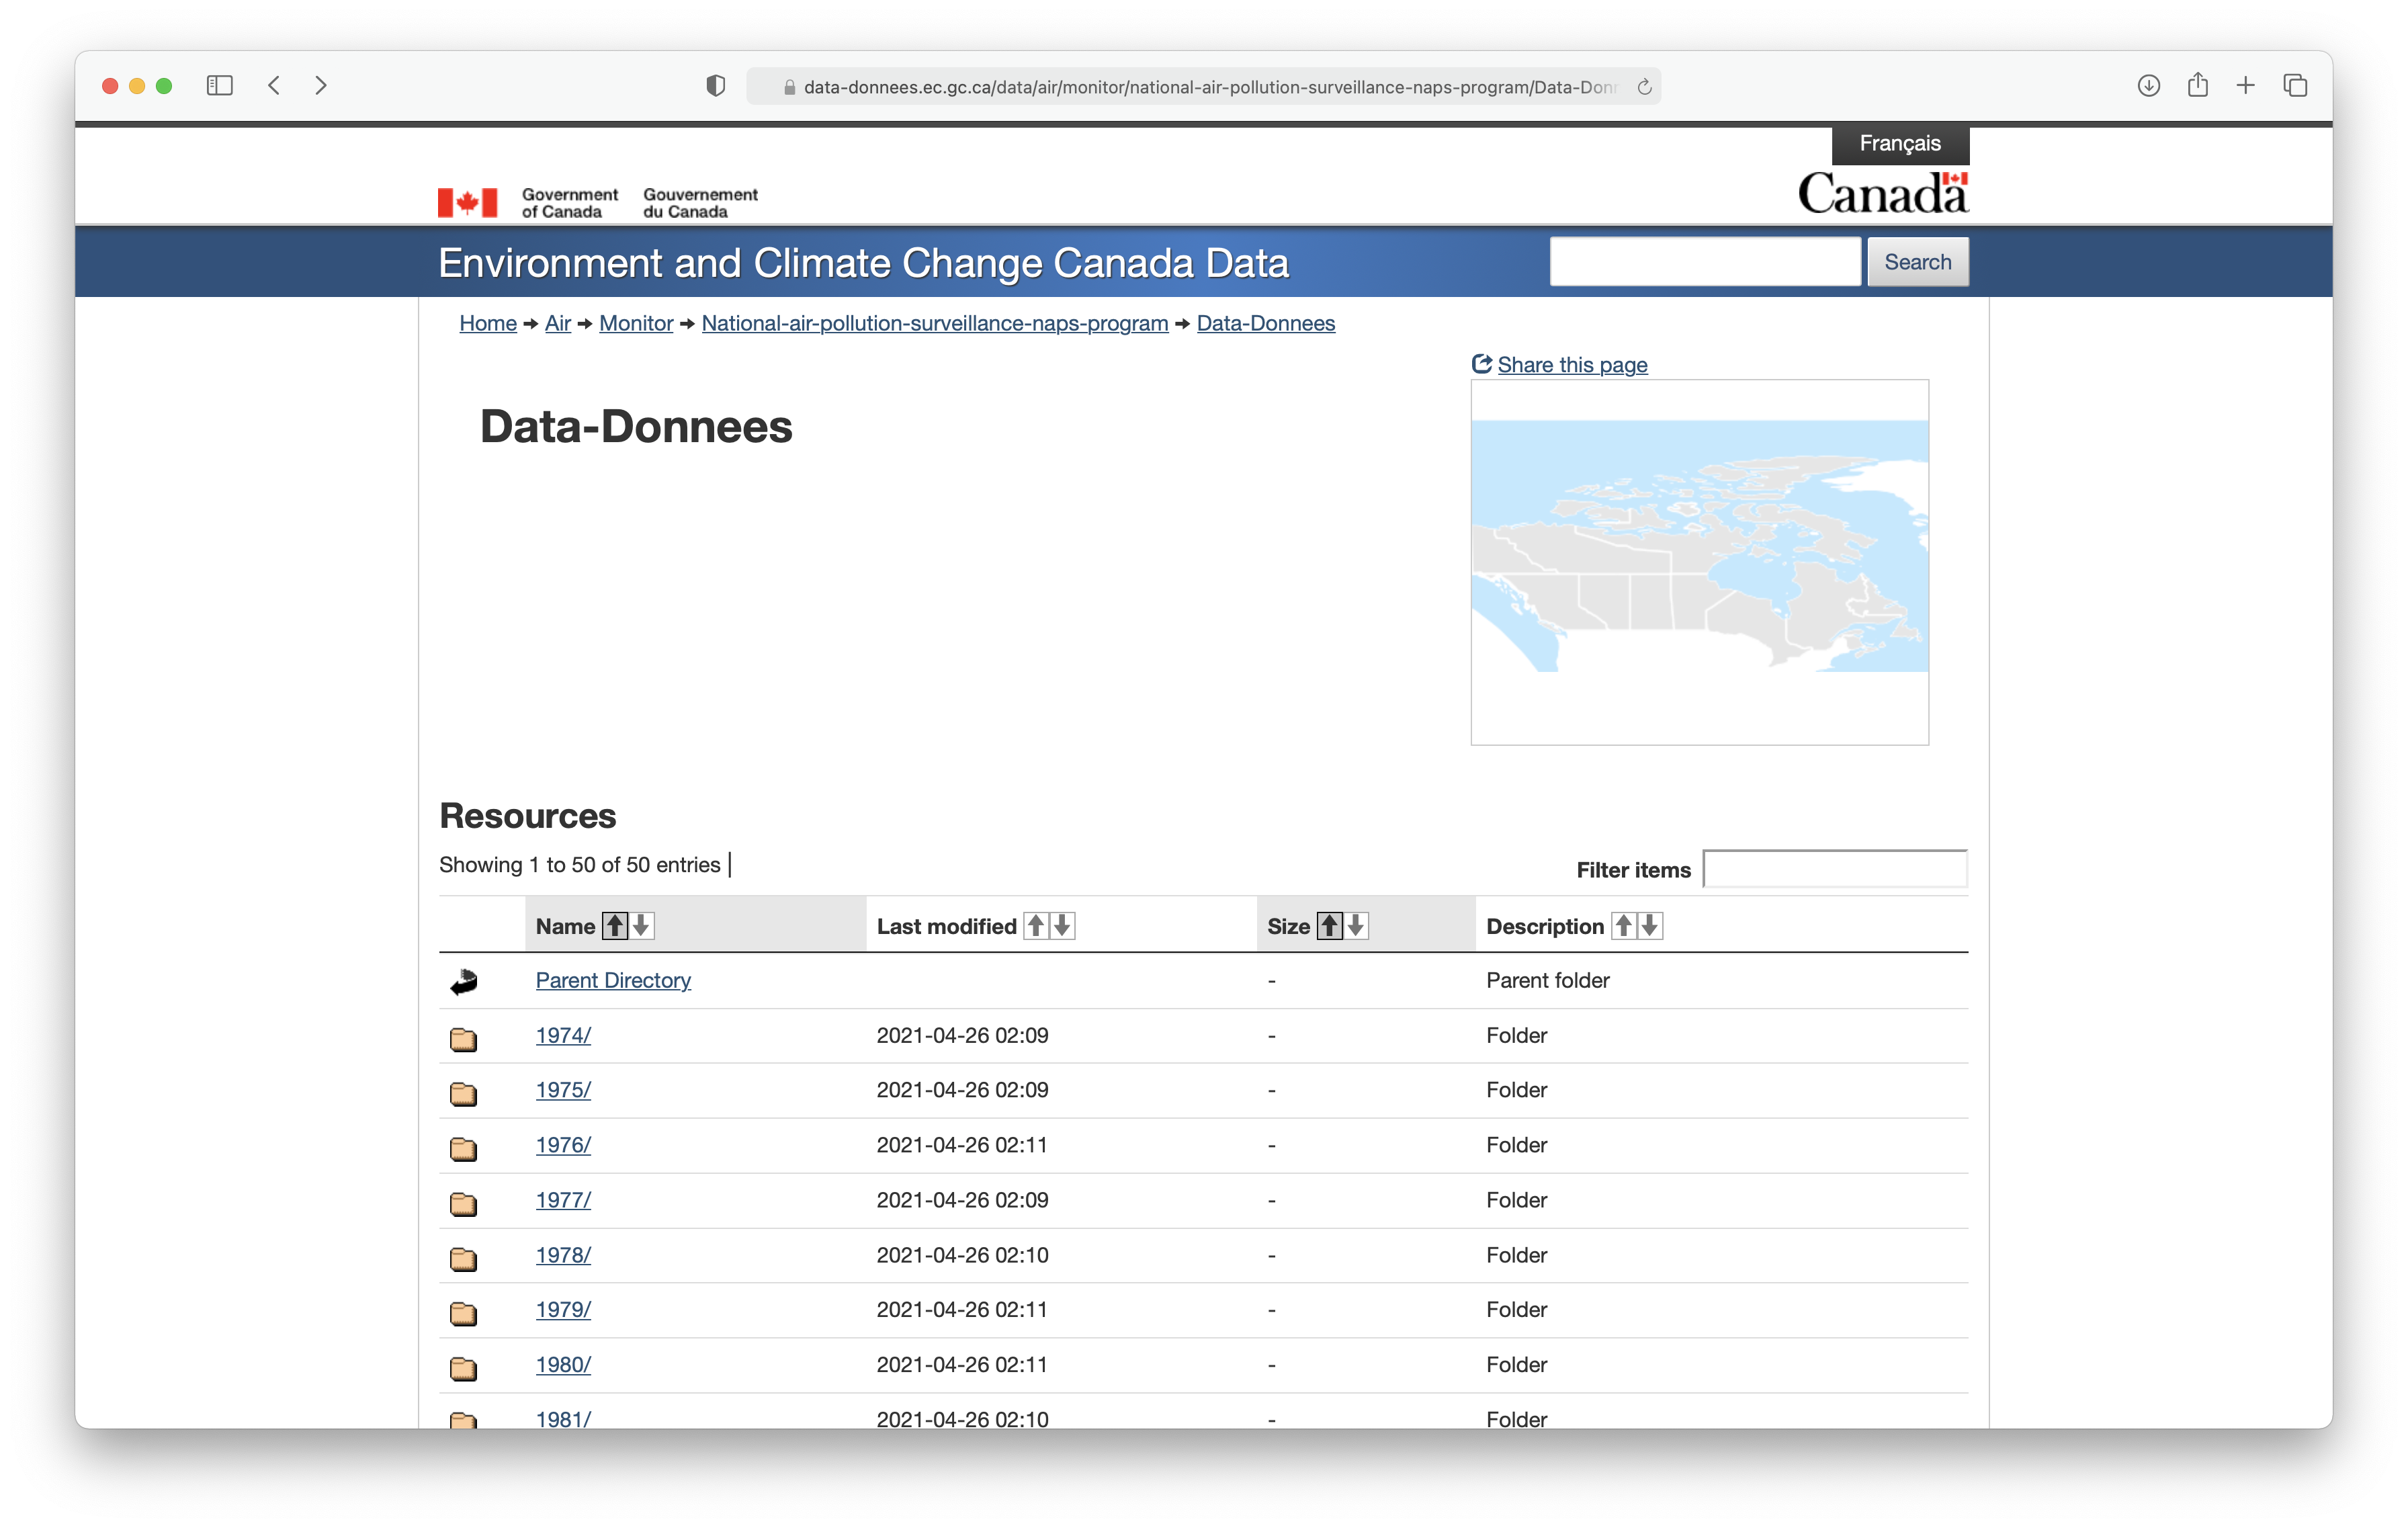
\includegraphics[width=\textwidth]{images/21-1-opendataset.png}
	\caption{NAPS Program: Live Open Dataset}
 \end{figure}

\newpage

\subsection*{Code Implementation}
The open dataset was provided in separate CSV files (by city) and was manually reorganized, cleansed and formatted into a single CSV table. The table was then summarized using an Excel pivot table and the data directly applied to a JavaScript data visualization framework (Plotly.js) displayed below to maximize data visualization speed and performance:

\begin{lstlisting}[language=java]
var trace1 = {
	x: ['AB', 'BC', 'MB', 'NB', 'NL', 'NS', 'ON', 'PE', 'QC', 'SK', 'YU'],
	y: [5.764, 4.922, 3.614, 5.668, 3.657, 3.674, 6.182, 3.321, 6.545, 4.722, 2.588],
	type: 'bar',
	text: ['5.764(micro)g/m3', '4.922(micro)g/m3', '3.614(micro)g/m3', '5.668(micro)g/m3', '3.657(micro)g/m3', '3.674(micro)g/m3', '6.182(micro)g/m3', '3.321(micro)g/m3', '6.545(micro)g/m3', '4.722(micro)g/m3', '2.588(micro)g/m3'],
	marker: { color: '#ffcc99' }
};

var data = [trace1];

var titleCode = `
	<span id="airQualityTitle" style="font-family: 'Public Sans', sans-serif; font-size: 1.618rem; font-weight: bold;">
		Statistic data of PM2.5 
	</span>
	<br>
	<span id="airQualitySubtitle" style="font-family: 'Public Sans', sans-serif; font-size: 1rem;">
		Based on National Air Pollution <br> Surveillance (NAPS) Program
	</span>
`;

var layout = {
	title: titleCode,
	font: { family: 'Raleway, sans-serif' },
	showlegend: false,
	xaxis: { tickangle: -45 },
	yaxis: {
		zeroline: false,
		gridwidth: 2
	},
	bargap: 0.5
};

Plotly.newPlot('airQuality', data, layout);
\end{lstlisting}

 \newpage

% =====================================================================
%   22. PHP
% =====================================================================
\section{PHP}

A minimum of 5 scripts with documentation and 26 total PHP scripts were created at the time of this writing to make the website fully-operational with its current features.
\begin{enumerate}
	\item \lstinline{DatabaseHelper.php}
	\item \lstinline{ThemeHelper.php}
	\item \lstinline{adminlogin_editrecord.php}
	\item \lstinline{adminlogin_edituser.php}
	\item \lstinline{adminlogin_status.php}
	\item \lstinline{adminlogout.php}
	\item \lstinline{city.php}
	\item \lstinline{dreamcity.php}
	\item \lstinline{editrecord.php}
	\item \lstinline{edituser.php}
	\item \lstinline{favorite.php}
	\item \lstinline{index.php}
	\item \lstinline{login.php}
	\item \lstinline{logout.php}
	\item \lstinline{navigation.php}
	\item \lstinline{post.php}
	\item \lstinline{profile.php}
	\item \lstinline{registration.php}
	\item \lstinline{status.php}
	\item \lstinline{switchtheme.php}
	\item \lstinline{userchange.php}
	\item \lstinline{validation_editrecord.php}
	\item \lstinline{validation_edituser.php}
	\item \lstinline{validation_status.php}
	\item \lstinline{validation.php}
\end{enumerate}

\newpage
\subsection*{5 PHP Script Samples with Documentation}

%   Script 1
% ------------------------------------------------------------------------

\begin{figure}[htbp]
	\centering
	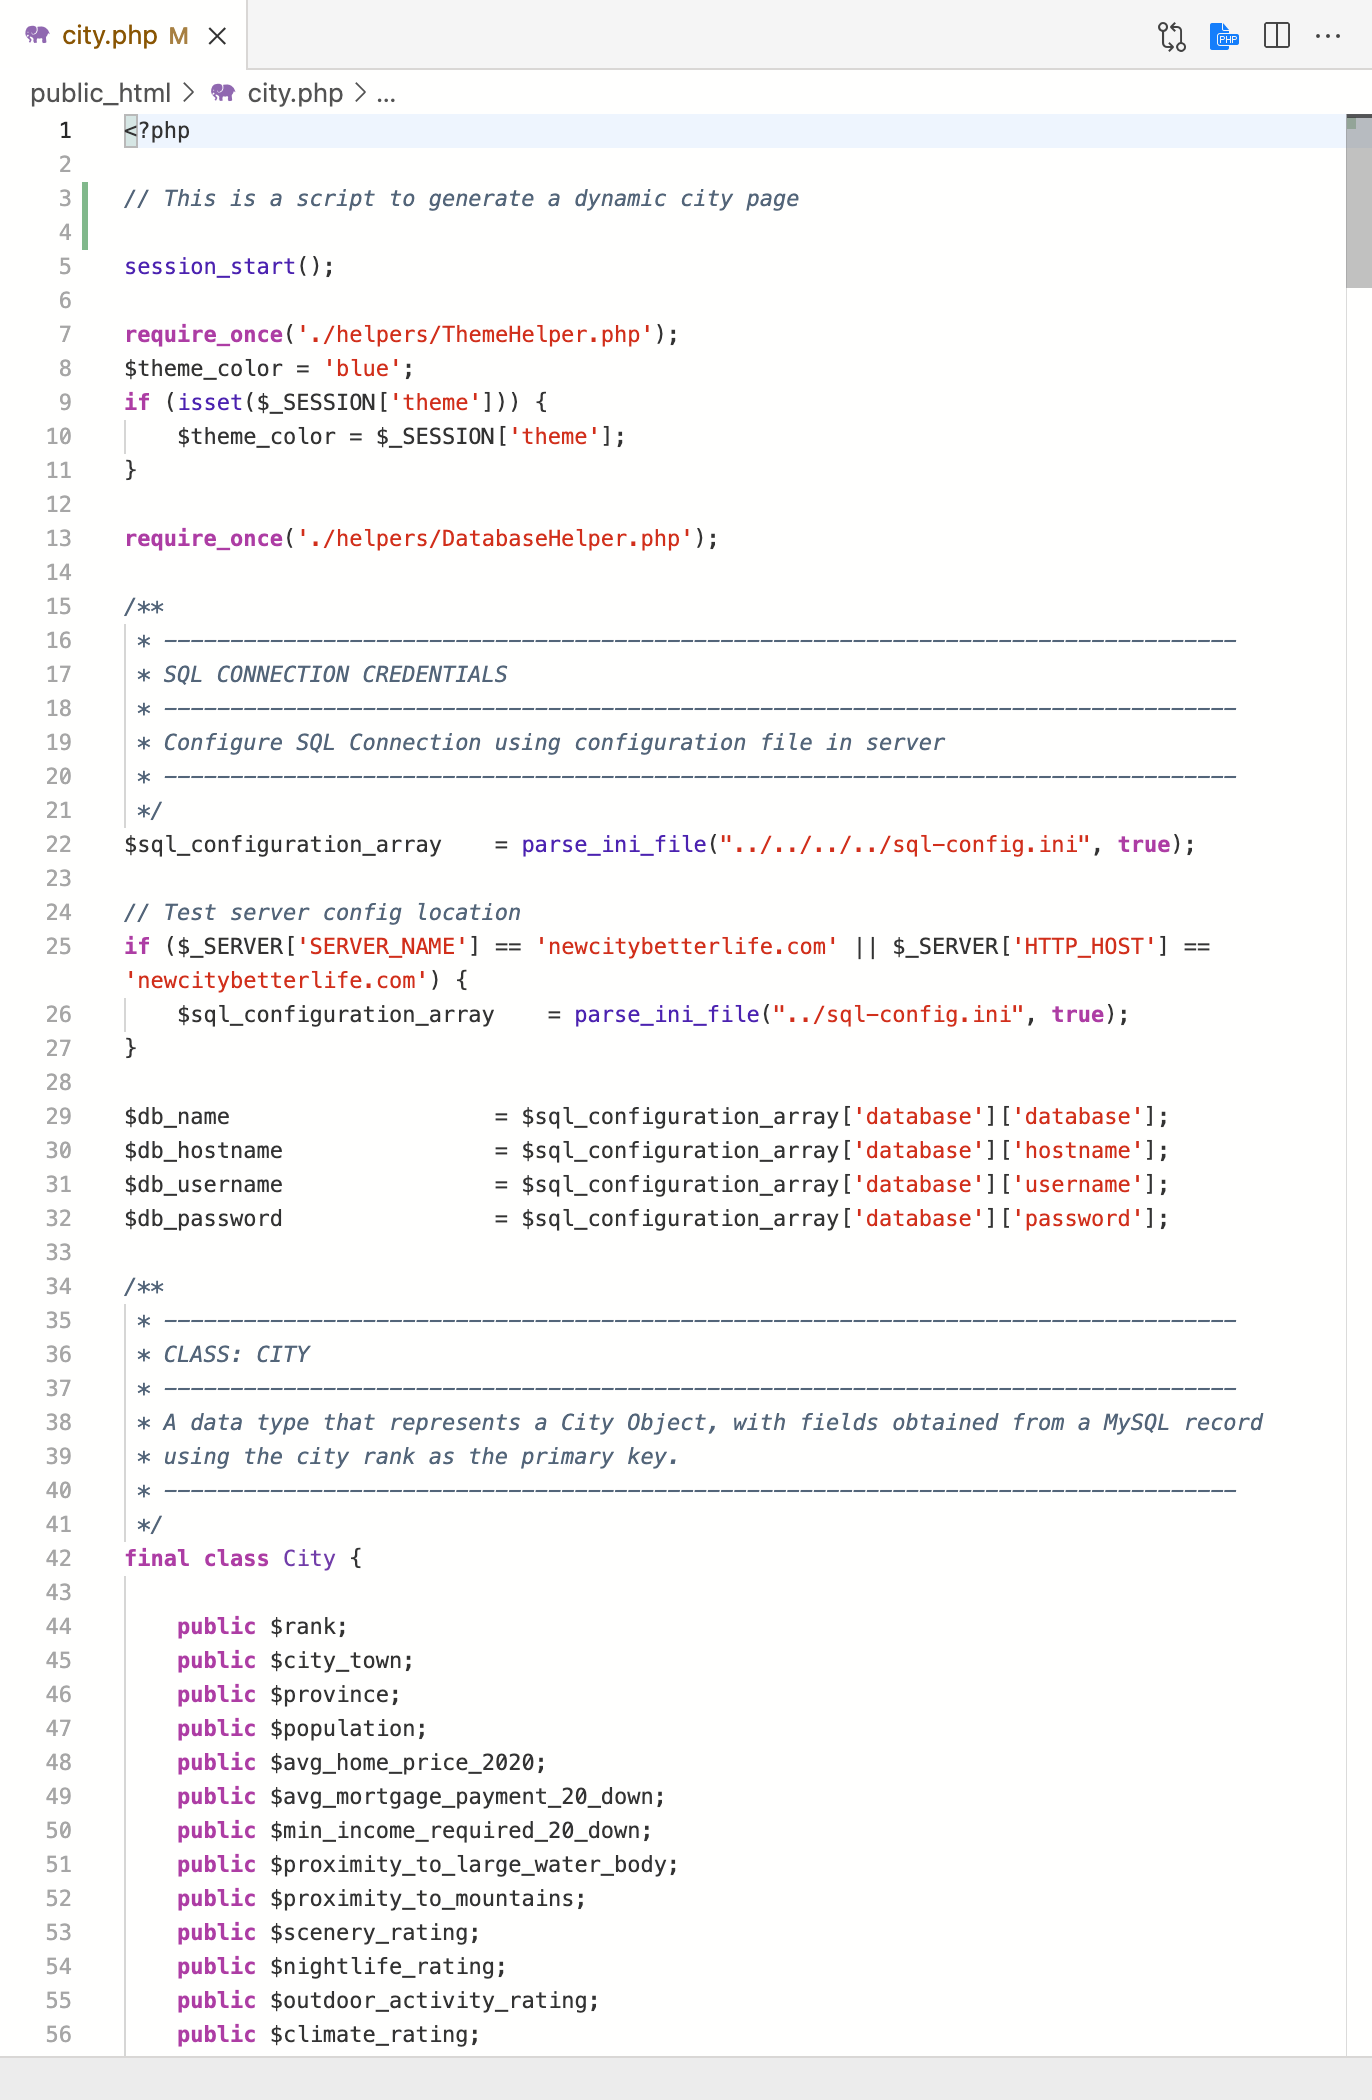
\includegraphics[width=4.3in]{images/22-script-1.png}
	\caption{Script: city.php}
 \end{figure}

 
%   Script 2
% ------------------------------------------------------------------------

\begin{figure}[htbp]
	\centering
	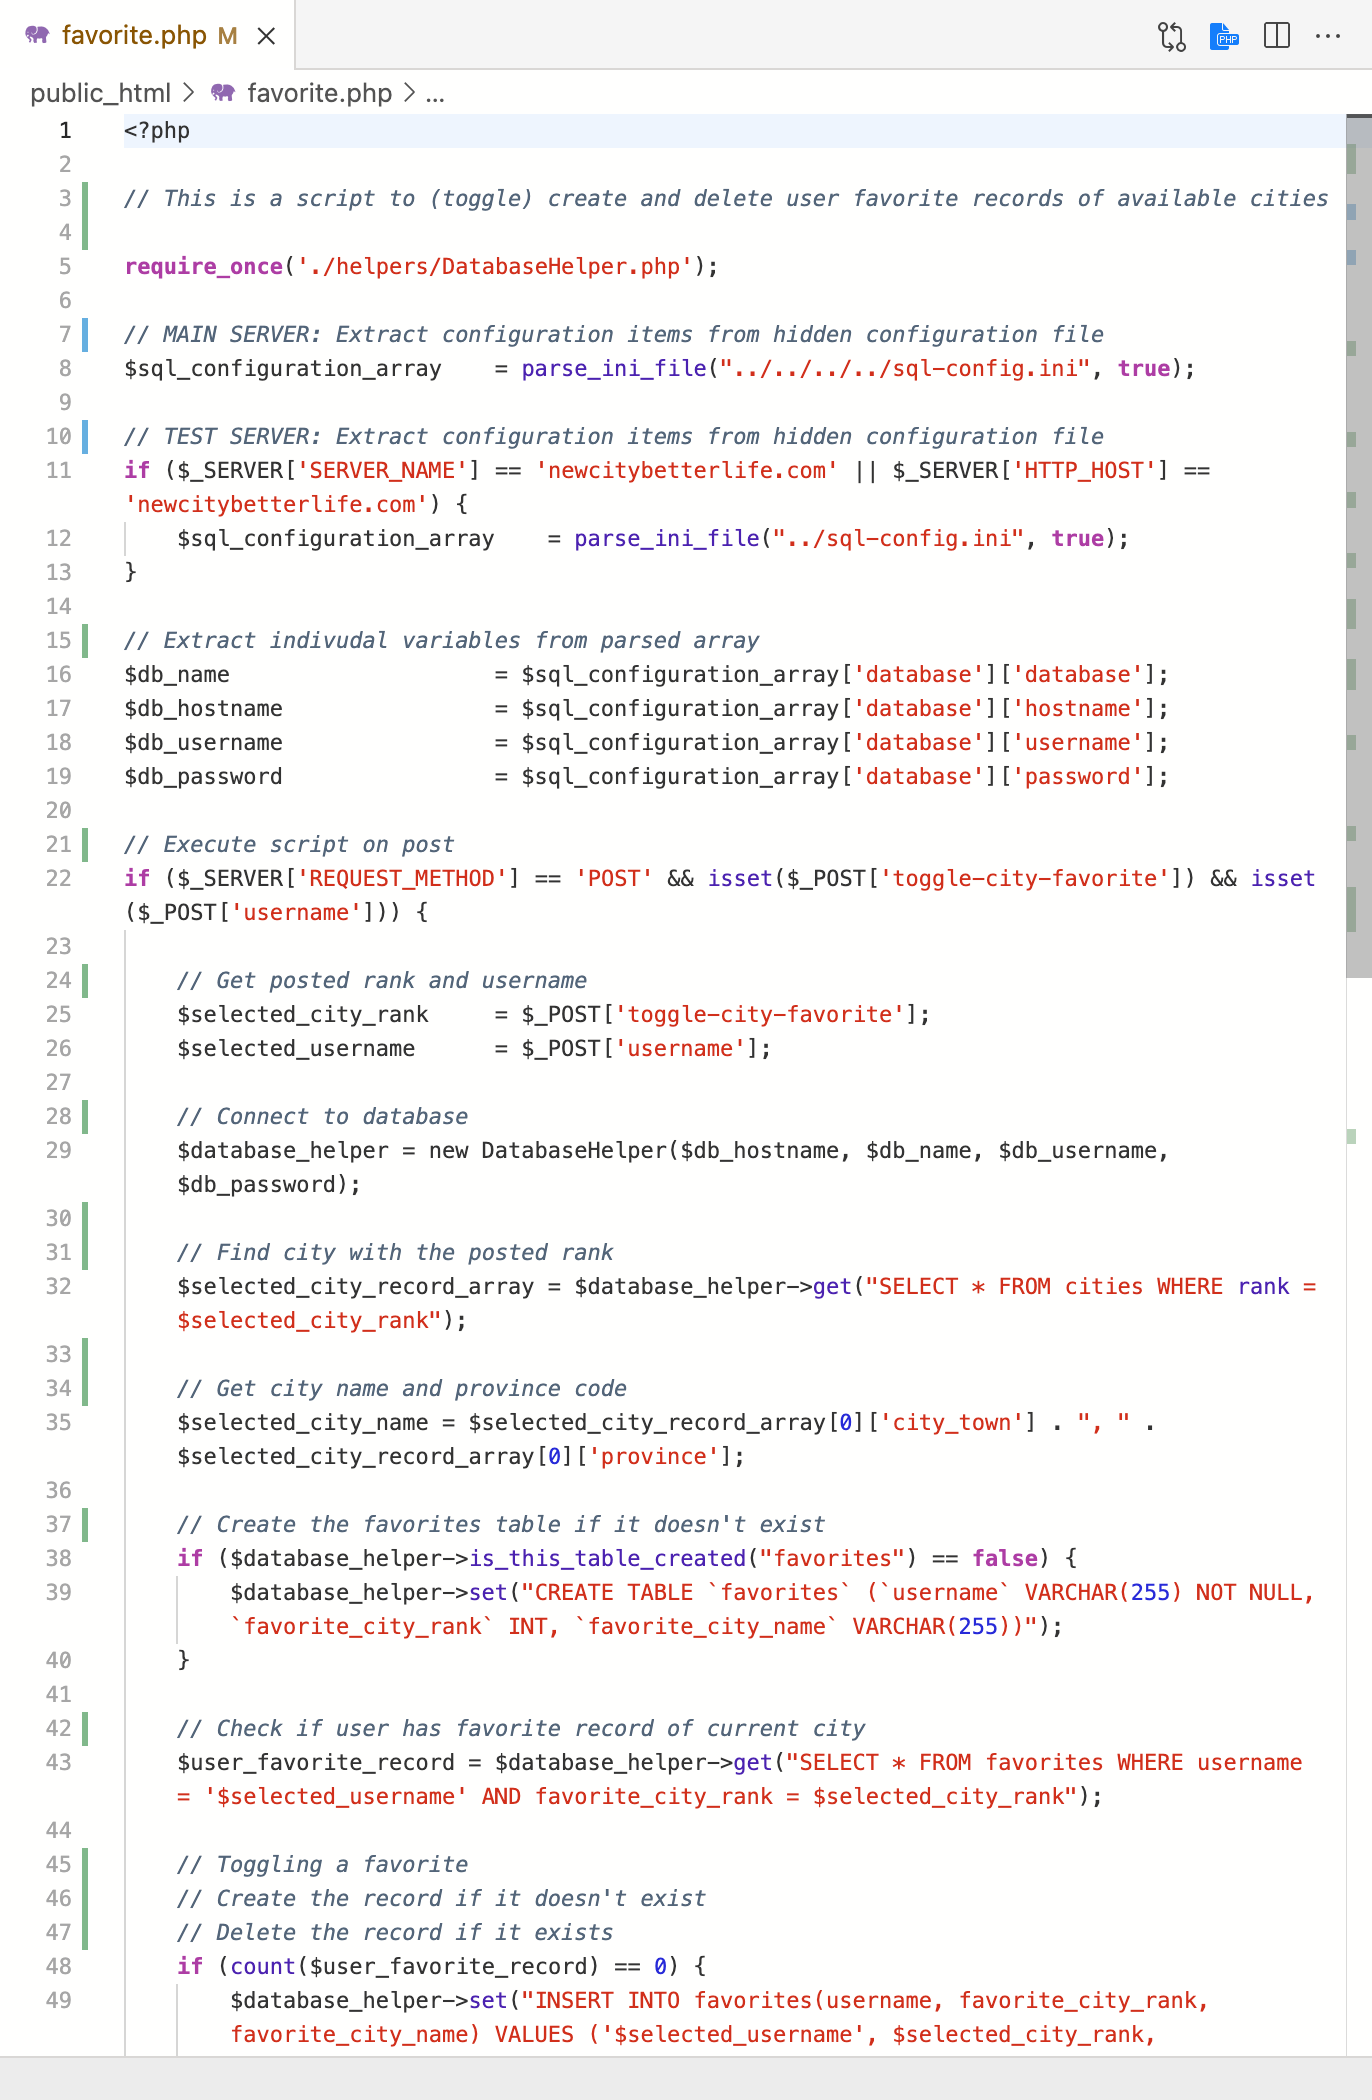
\includegraphics[width=4.3in]{images/22-script-2.png}
	\caption{Script: favorite.php}
 \end{figure}

%   Script 3
% ------------------------------------------------------------------------

\begin{figure}[htbp]
	\centering
	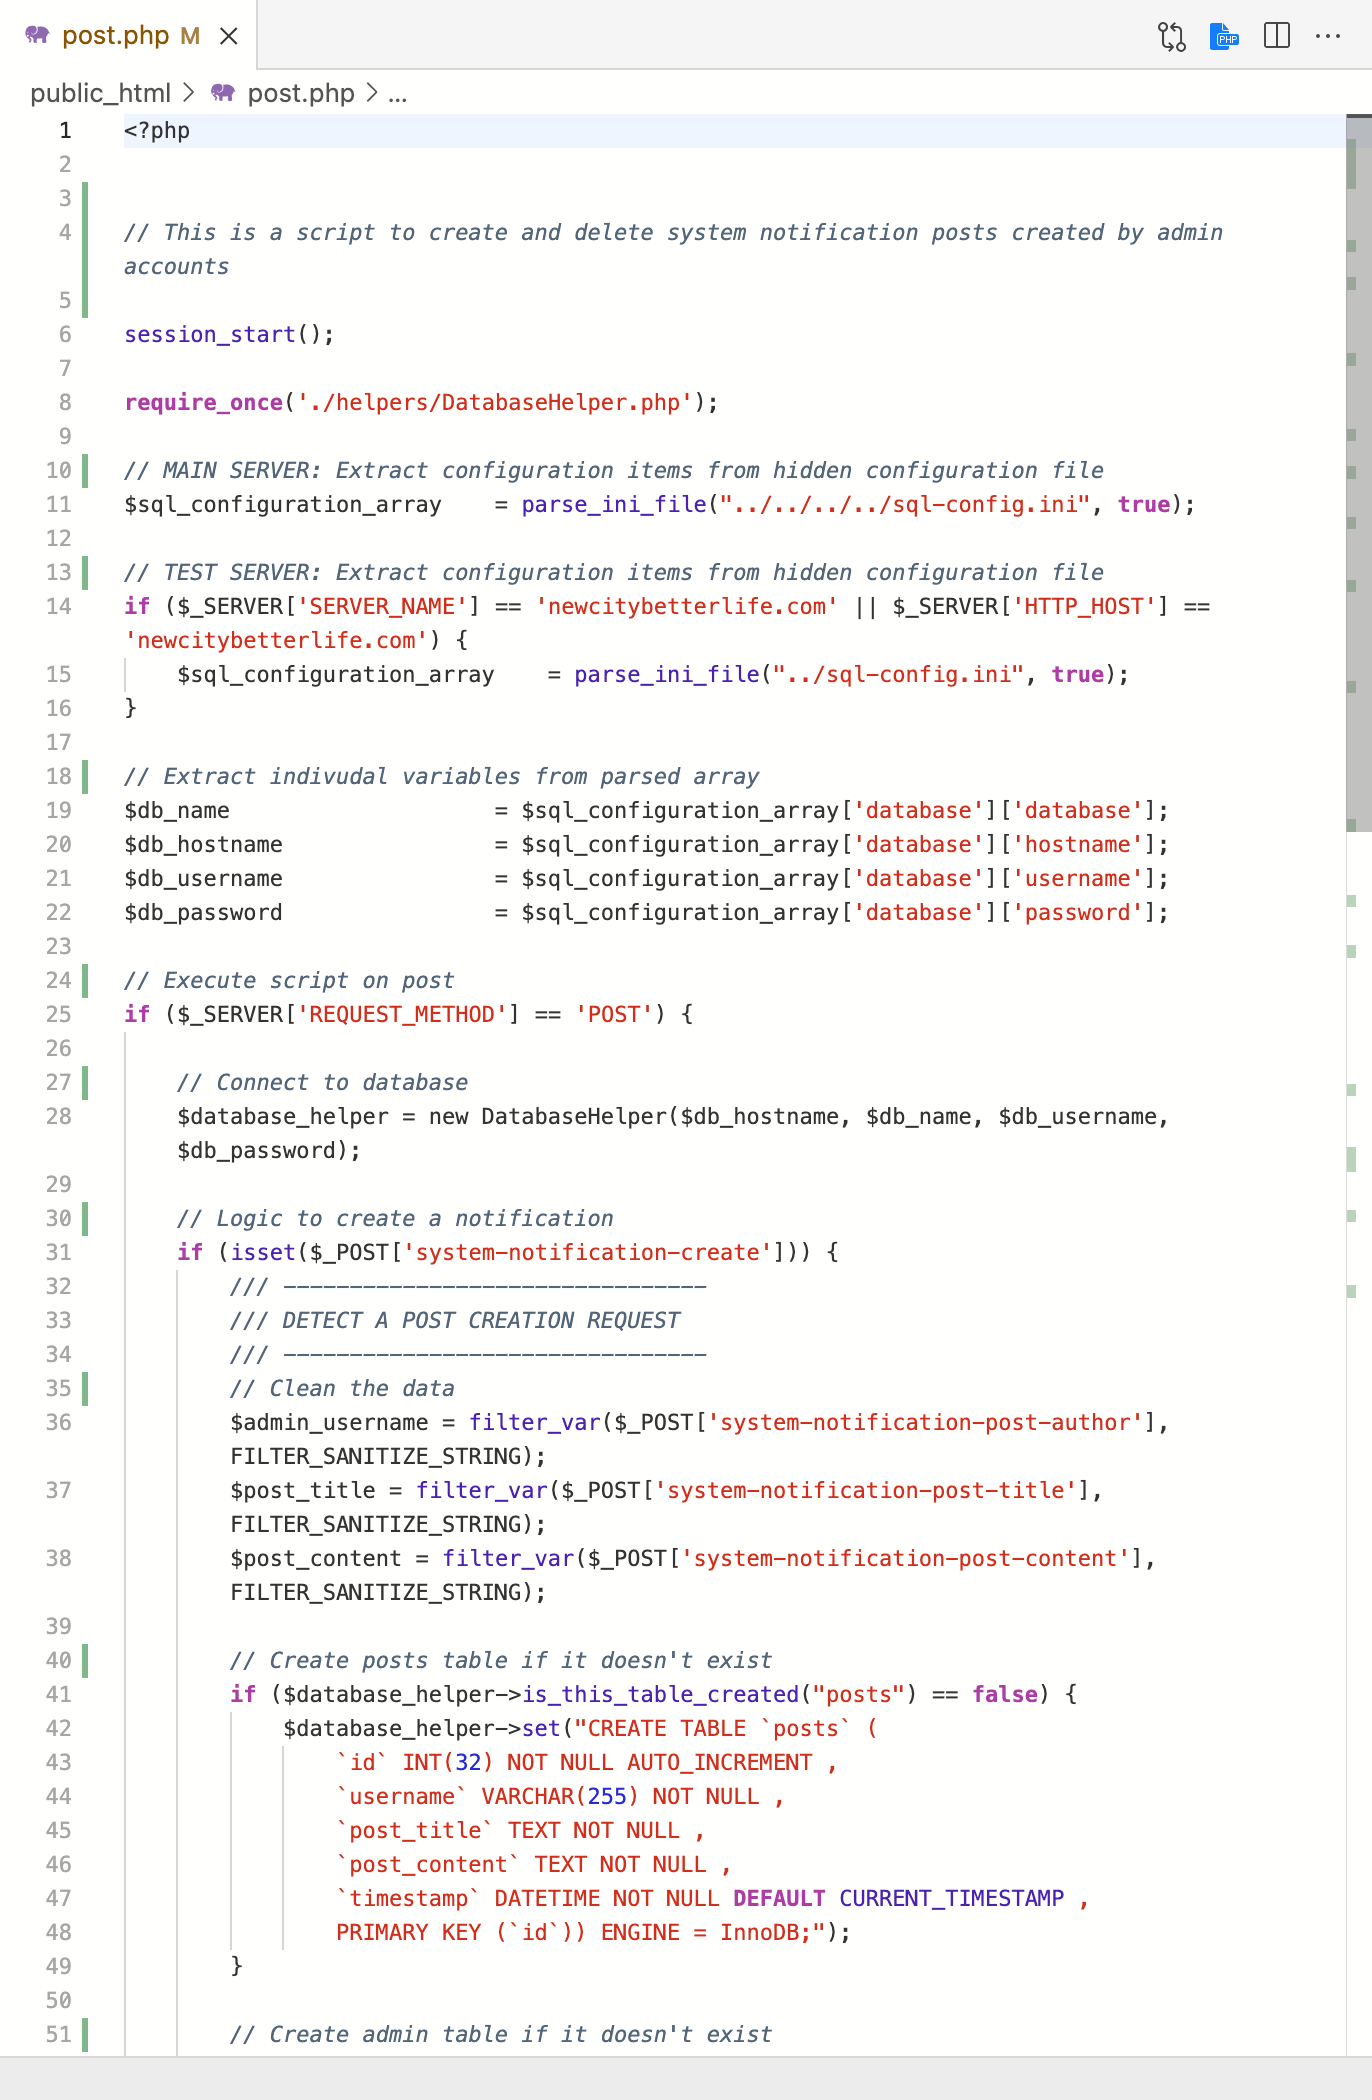
\includegraphics[width=4.3in]{images/22-script-3.png}
	\caption{Script: post.php}
 \end{figure}

%   Script 4
% ------------------------------------------------------------------------

\begin{figure}[htbp]
	\centering
	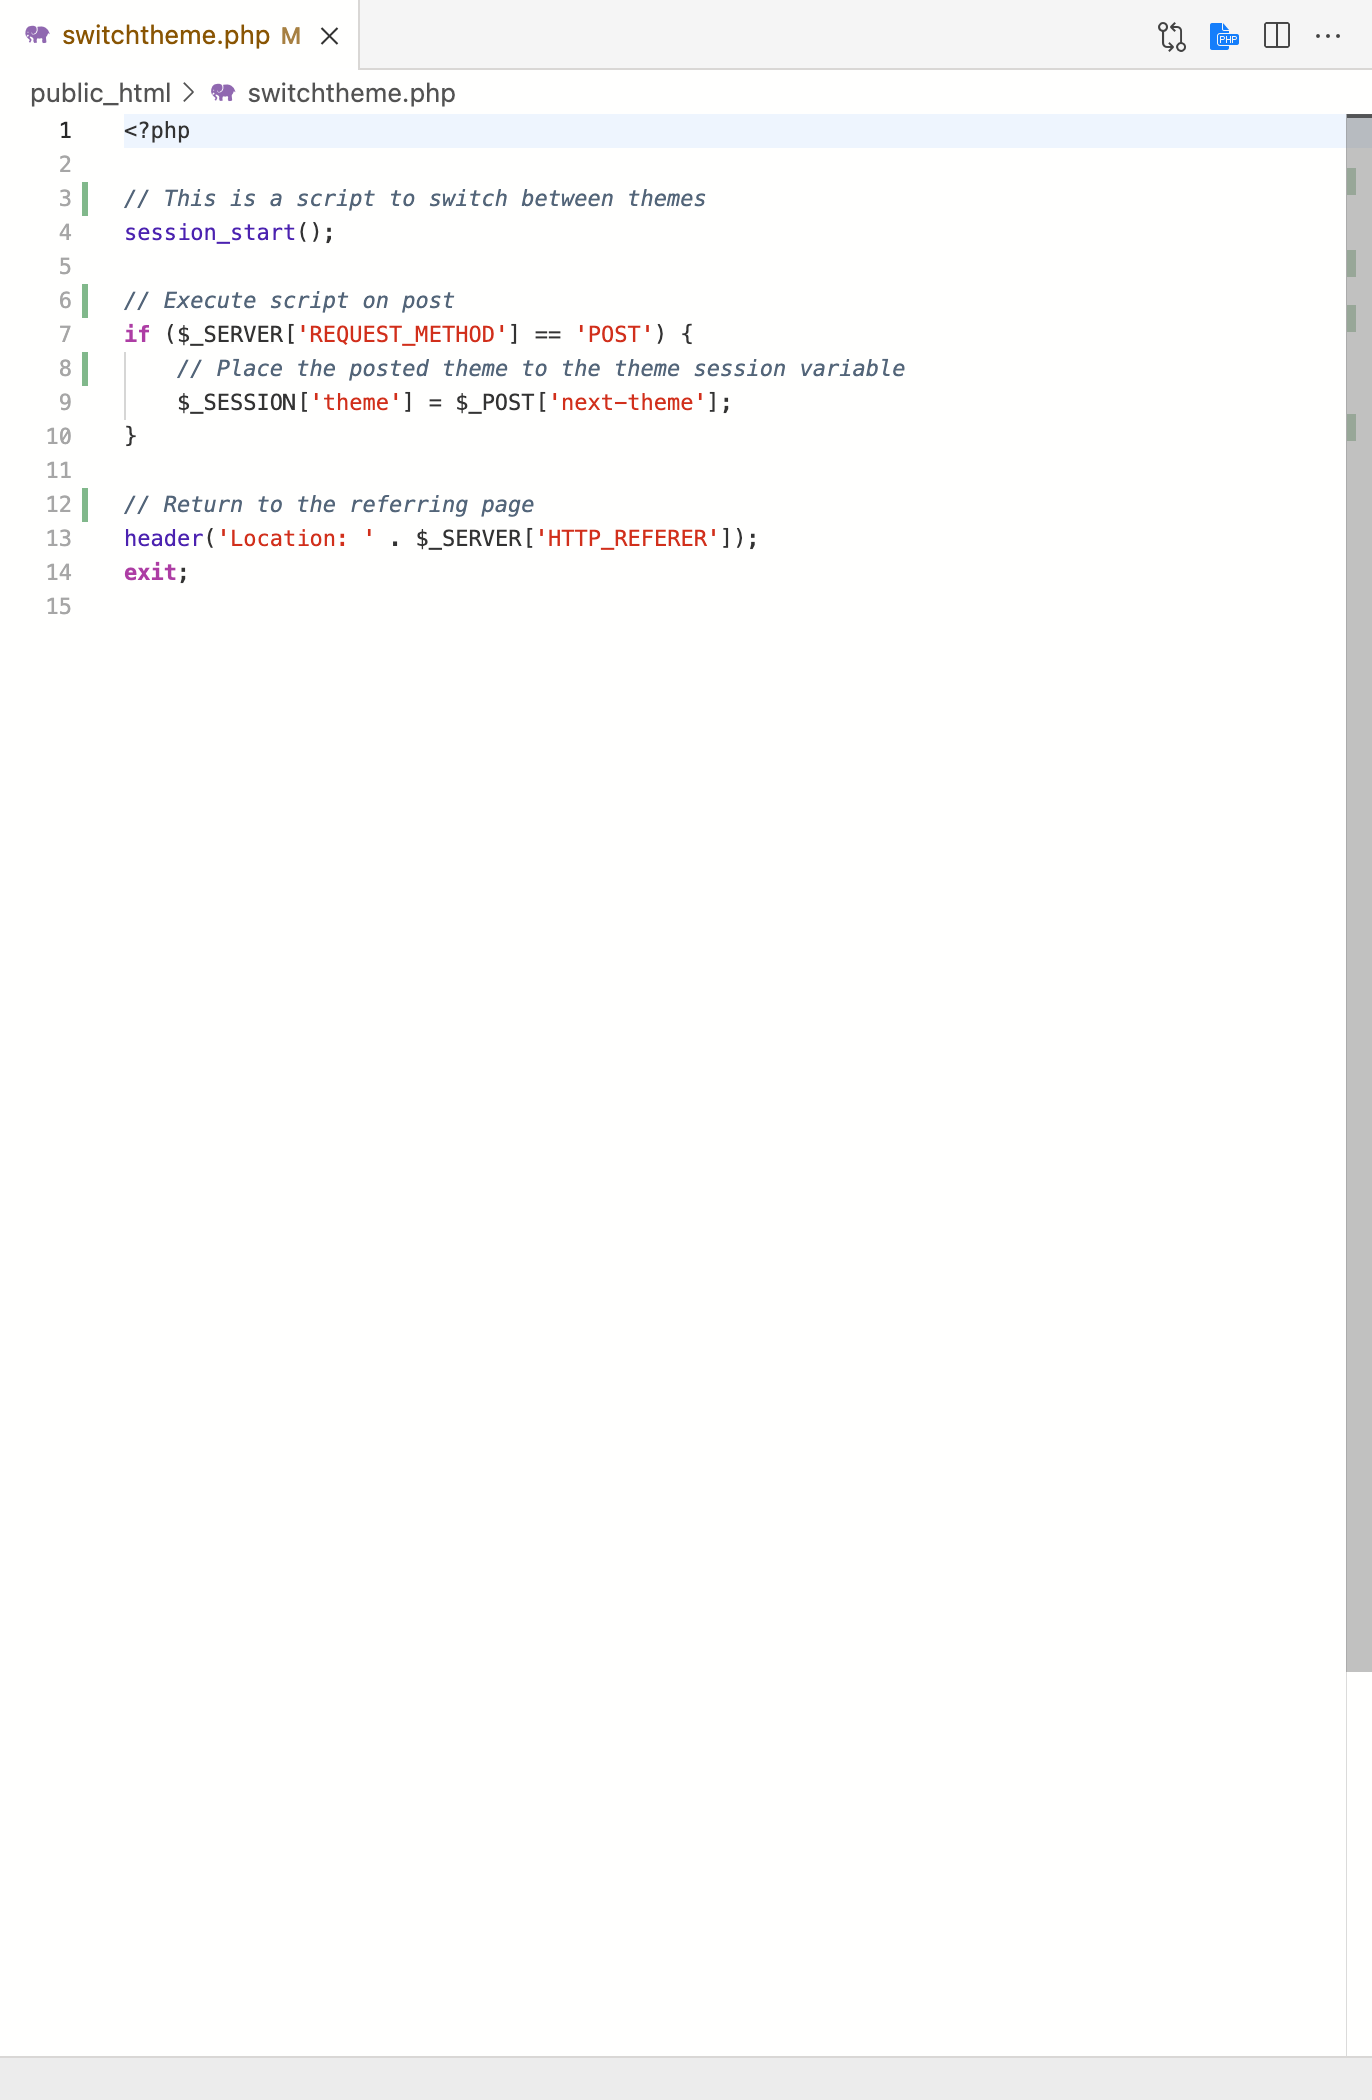
\includegraphics[width=4.3in]{images/22-script-4.png}
	\caption{Script: switchtheme.php}
 \end{figure}

%   Script 5
% ------------------------------------------------------------------------

\begin{figure}[htbp]
	\centering
	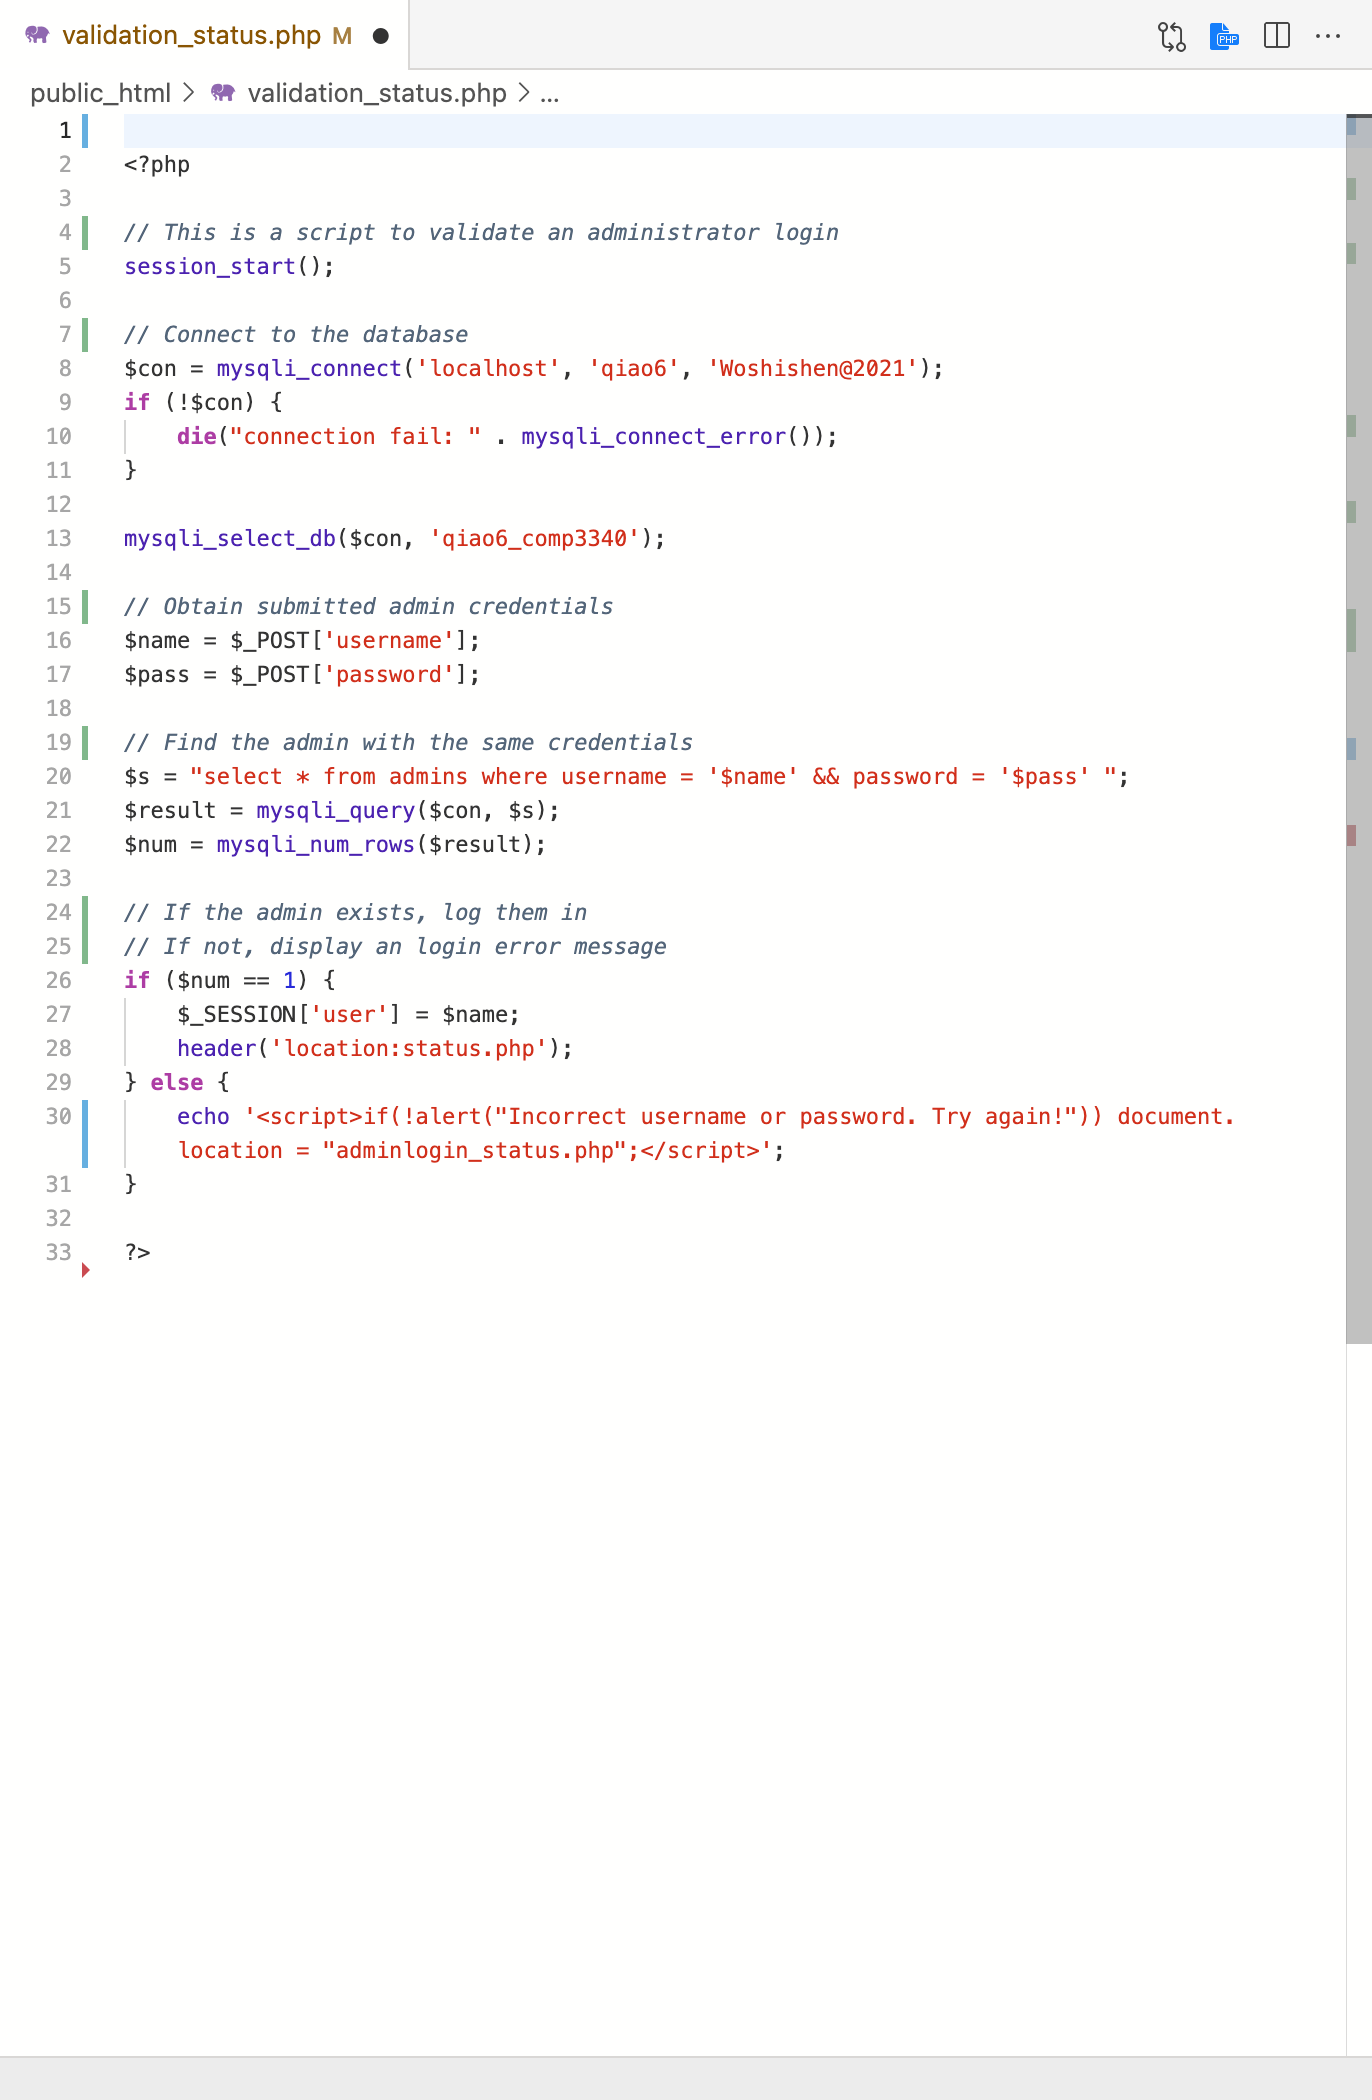
\includegraphics[width=4.3in]{images/22-script-5.png}
	\caption{Script: validation\_status.php}
 \end{figure}

 \newpage

% =====================================================================
%   23. ADDITIONAL LANGUAGE / FRAMEWORK
% =====================================================================
\section{Additional Language/Framework}
we created 11 reactJS scripts

In your report, for each item using the corresponding section number from the table above to present/expand on the work you have done. You can include code segments, screenshots and charts as needed for each individual section. You will receive points as indicated above for each section. There is no page limit. Keep the screenshots readable.

up to 5 pts for non-trivial use of another language/framework

\begin{figure}[htbp]
	\centering
	
\includegraphics[width=3in]{images/placeholder.jpg}
	\caption{Caption Goes Here}
 \end{figure}

 \newpage

% =====================================================================
%   24. SOFTWARE REPOSITORY
% =====================================================================
\section{Software Repository}
we used github here is the link: url here (be sure to provide public access to it; or a guest username/password)

In your report, for each item using the corresponding section number from the table above to present/expand on the work you have done. You can include code segments, screenshots and charts as needed for each individual section. You will receive points as indicated above for each section. There is no page limit. Keep the screenshots readable.

up to 5 pts for showing a thorough repository with multiple branches/history

\begin{figure}[htbp]
	\centering
	
\includegraphics[width=3in]{images/placeholder.jpg}
	\caption{Caption Goes Here}
 \end{figure}

 \newpage

% =====================================================================
%   25. INSTALLATION AND DEPLOYMENT
% =====================================================================
\section{Installation and Deployment}
this site can be cloned from the github repository using the following branch, with instructions to configure the db manually found here: url here

In your report, for each item using the corresponding section number from the table above to present/expand on the work you have done. You can include code segments, screenshots and charts as needed for each individual section. You will receive points as indicated above for each section. There is no page limit. Keep the screenshots readable.

up to 2 pts for installation instructions

\begin{figure}[htbp]
	\centering
	
\includegraphics[width=3in]{images/placeholder.jpg}
	\caption{Caption Goes Here}
 \end{figure}

 \newpage

% =====================================================================
%   26. ACCESSIBILITY
% =====================================================================
\section{Accessibility}
we used tags for all images, and ensure compliance with WCAG2.0 standard (url)  tool used: .. Link: HTTP:../ report attached.

In your report, for each item using the corresponding section number from the table above to present/expand on the work you have done. You can include code segments, screenshots and charts as needed for each individual section. You will receive points as indicated above for each section. There is no page limit. Keep the screenshots readable.

up to 5 pts for the report printout showing compliance for the site

\begin{figure}[htbp]
	\centering
	
\includegraphics[width=3in]{images/placeholder.jpg}
	\caption{Caption Goes Here}
 \end{figure}

 \newpage

% =====================================================================
%   27. MARK-UP VALIDATION SERVICE
% =====================================================================
\section{Mark-Up Validation Service}

Ran the site on: https://validator.w3.org/

report attached

In your report, for each item using the corresponding section number from the table above to present/expand on the work you have done. You can include code segments, screenshots and charts as needed for each individual section. You will receive points as indicated above for each section. There is no page limit. Keep the screenshots readable.

up to 5 pts for the report printout showing compliance for the site.

\begin{figure}[htbp]
	\centering
	
\includegraphics[width=3in]{images/placeholder.jpg}
	\caption{Caption Goes Here}
 \end{figure}

 \newpage

% =====================================================================
%   28. TESTING
% =====================================================================
\section{Testing}
used selenium to test for broken links and a bug reporting tool on redmine. (testing tool not required; but any form of testing is expected, at least one)

In your report, for each item using the corresponding section number from the table above to present/expand on the work you have done. You can include code segments, screenshots and charts as needed for each individual section. You will receive points as indicated above for each section. There is no page limit. Keep the screenshots readable.

up to 5 pts for a testing strategy

\begin{figure}[htbp]
	\centering
	
\includegraphics[width=3in]{images/placeholder.jpg}
	\caption{Caption Goes Here}
 \end{figure}

 \newpage

% =====================================================================
%   29. TEAM MANAGEMENT
% =====================================================================
\section{Team Management}
We used redmine for team management link here be sure to provide guest access or plenty of screenshots

In your report, for each item using the corresponding section number from the table above to present/expand on the work you have done. You can include code segments, screenshots and charts as needed for each individual section. You will receive points as indicated above for each section. There is no page limit. Keep the screenshots readable.

up to 5 pts for team work organized over a period of no less than 4 weeks

\begin{figure}[htbp]
	\centering
	
\includegraphics[width=3in]{images/placeholder.jpg}
	\caption{Caption Goes Here}
 \end{figure}

 \newpage

% =====================================================================
%   30. OVERALL COMPLETENESS AND ERROR FREE FUNCTIONALITY
% =====================================================================
\section{Overall Completeness \& Error Free Functionality}
Site can be tested here, we completed 100 percent of the functionality here is the sitemap showing all the features

In your report, for each item using the corresponding section number from the table above to present/expand on the work you have done. You can include code segments, screenshots and charts as needed for each individual section. You will receive points as indicated above for each section. There is no page limit. Keep the screenshots readable.

up to 10 pts for overall impression of the site in terms of complete functionality and error free (aesthetics / look and feel are not given grades, but CSS use is expected).

\begin{figure}[htbp]
	\centering
	
\includegraphics[width=3in]{images/placeholder.jpg}
	\caption{Caption Goes Here}
 \end{figure}


\end{document}